\section{Umsetzung}
\label{sec:chapterRealization}

In diesem Hauptkapitel werden Details zur Umsetzung dokumentiert. Hier sind Konfigurationen, Technologiebeschreibungen, Code Listings und sonstige technische Erklärungen über openHAB, MQTT und die Android App zu finden.


\subsection{openHAB Konfiguration}
Items, Rules, Sitemaps und Persitence Strategies werden in openHAB in einer eigens dafür entwickelten DSL beschrieben. Für alle diese Bereiche werden Konfigurationsdateien im entsprechenden Unterverzeichnis des openHAB Konfigurationsordner abgelegt. Änderungen an den Konfigurationsdateien werden von openHAB zur Laufzeit sofort erkannt und berücksichtigt. Nebst den genannten Bereichen existiert noch eine globale Konfigurationsdatei um beispielsweise IP-Adressen für Bindings einzutragen. Folgende Dateien sind für diese Arbeit relevant:

\begin{itemize}
	\item /configurations/*.cfg
	\item /configurations/items/*.items
	\item /configurations/rules/*.rules
	\item /configurations/sitemaps/*.sitemap
	\item /configurations/persistence/*.persist
	\item /configurations/transform/*.map
\end{itemize}

Anhand diesen Konfigurationen werden die User Cases modelliert.

\subsubsection{Konfiguration Überwachungskamera} 
Für die Überwachungskamera existiert kein entsprechendes Item. Stattdessen wird in der Sitemap ein Image-Element angezeigt, dessen URL auf das HTTP Snapshot Interface der Netzwerkkamera verweist.\\ \\
Das Bild wird dank dem Attribut \lstinline!visibility!  immer dann angezeigt, wenn das Item \lstinline!Alarm_activated! den Wert \lstinline!ON! hat. Das \lstinline!refresh! Interval bewirkt einen Reload des Bildes alle 200 Millisekunden.

\begin{lstlisting}[style=csharp, caption=demo.sitemap - Webcam Bild]
[...]
Image url="http://192.168.1.15/snapshot.jpg" refresh=200
visibility=[Alarm_activated==ON]
[...]
\end{lstlisting}




\subsubsection{Konfiguration Kontaktsensor} 
Der Kontaktsensor ist ein Use Case der in openHAB sehr oft vorkommt. Deshalb existiert ein Item Type «Contact» mit den beiden möglichen Werten OPEN und CLOSED. Das Homematic Binding liefert aber die Werte \lstinline!true! oder \lstinline!false! und kann deshalb nicht an ein Contact Item gebunden werden. Als Alternative haben wir ein String Item verwendet und mit Hilfe einer Transformation-Map \lstinline!false! mit «geschlossen» und \lstinline!true! mit «offen» übersetzt. Das Icon <contact> kann trotzdem noch verwendet werden. Allerdings wird nun nicht mehr automatisch das Icon für das offene bzw. geschlossene Fenster angezeigt, da openHAB den Basisnamen des Icons mit dem State konkateniert. Wir haben dementsprechend die Icons kopiert und ein File contact-false.png und contact-true.png im Ressourcen-Ordner hinterlegt.\\ \\
Auf der letzten Zeile werden die Bindingparameter für Homematic angegeben.\\ \lstinline!address=LEQ1469091! bezieht sich auf die Seriennummer des Kontaktsensors und\\ \lstinline!parameter=STATE! gibt an, welche Eigenschaft gebunden werden soll. \lstinline!channel=1! ist ein Defaultwert.

\begin{lstlisting}[style=csharp, caption=demo.items - Kontaktsensor]
[...]
String Window_Bedroom "Schlafzimmerfenster [MAP(window.map):%s]"
<contact> (OV_Windows, Windows)
{homematic="address=LEQ1469091,channel=1,parameter=STATE"}
[...]
\end{lstlisting}

In der Sitemap wird das Item in einem Text-Element referenziert. Weitere Attribute sind nicht notwendig.

\begin{lstlisting}[style=csharp, caption=demo.sitemap - Kontaktsensor]
[...]
Text item=Window_Bedroom
[...]
\end{lstlisting}

\subsubsection{Konfiguration Bewegungsmelder}
Der Bewegungsmelder ist ebenfalls von Homematic und wird in den Bindingparametern gleich referenziert wie beim Kontaktsensor. Der Bindingparameter \lstinline!MOTION! erhält einen boolschen Wert und muss mit Hilfe der Map \lstinline!motion.map! in einen benutzerfreundlichen String transformiert werden. Der Parameter \lstinline!ERROR! dient dem Sabotageschutz.\\ \\
Leider muss bei Homematic jeder Parameter einem eigenen Item zugeordnet werden. Deshalb haben wir ein drittes String-Item \lstinline!Motion_Summary! definiert, indem die Werte der beiden anderen Items zusammengefasst werden. 


\begin{lstlisting}[style=csharp, caption=demo.items - Bewegungsmelder Items]
[...]
String Motion_Livingroom "Bewegungsmelder [MAP(motion.map):%s]"
{homematic="address=LEQ0797607, channel=1, parameter=MOTION"}

String Motion_Livingroom_Sabotage "Sabotage"
{homematic="address=LEQ0797607, channel=1, parameter=ERROR"}

String Motion_Summary "Bewegungsmelder [%s]"
[...]
\end{lstlisting}

Die Ermittlung und Zuweisung des korrekten Wertes an das Item \lstinline!Motion_Summary! geschieht mit Hilfe der Rule \lstinline!Motion Aggregator!, die im nächsten Abschnitt erklärt wird.

\subsubsection{Rules}
Wie im Lösungskonzept beschrieben, werden Rules zur Automatisierung von Aktionen eingesetzt. Die Regeln können im File \lstinline!/etc/openhab/configurations/rules/demo.rules! definiert werden. \\\\
\textbf{Alarm} \\
In der Grafik \ref{fig:flowchartAlarm} wird der Ablauf der Alarm-Regel gezeigt. Im Wesentlichen geht es darum, beim Erkennen von Bewegung und offenem Fenster das Licht einzuschalten und die aufgenommenen Bilder der Webcam zu speichern. Dies soll jedoch nur geschehen, wenn der Alarm eingeschaltet ist.
\begin{figure}[H]
	\centering
		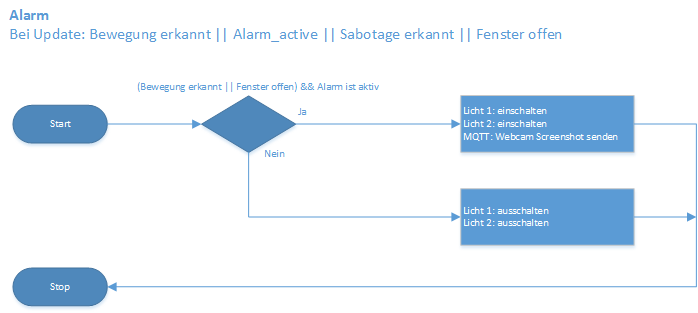
\includegraphics[scale=0.8]{report/img/RuleAlarm}
	\caption{Flowchart Alarm Rule}
	\label{fig:flowchartAlarm}
\end{figure}

Umgesetzt wird diese Flowchart durch folgenden Code. Diese Rules sind in der von openHAB selbst definierten DSL (Domain Specific Language) geschrieben.

\begin{lstlisting}[style=csharp, caption=demo.rules - Rule «Motion Aggregator»]
rule "Alarm"
	when Item Motion_Livingroom received update or
	     Item Motion_Livingroom_Sabotage received update or
	     Item Window_Bedroom received update
	then
	if(Motion_Livingroom.state == "true" ||
	   Window_Bedroom.state == "true") {
		sendCommand(Hue_1, ON)
		sendCommand(Hue_2, ON)
		sendMqttFile("openhab/blob",
					 "http://192.168.1.15/snapshot.jpg")
	} else {
		sendCommand(Hue_1, OFF)
		sendCommand(Hue_2, OFF)
	}
end
\end{lstlisting}

\textbf{Bewegungsmelder Aggregation} \\
Diese Regel definiert die verschiedenen Status, die der Bewegungsmelder haben kann. Durch diese Regel wird der aktuelle Status ermittelt und für das Item \lstinline!Motion_Summary! gesetzt. \\
Da der Bewegungsmelder Bewegungen und Sabotage erkennen kann (wenn die Halterung entfernt wird), ergeben sich vier mögliche Zustände: «Ruhig», «Bewegung erkannt», «Bewegung und Sabotage erkannt» und «Sabotage erkannt».\\
In der Abbildung \ref{fig:flowChartMotionAggregator} wird der Ablauf illustriert.

\begin{figure}[H]
	\centering
		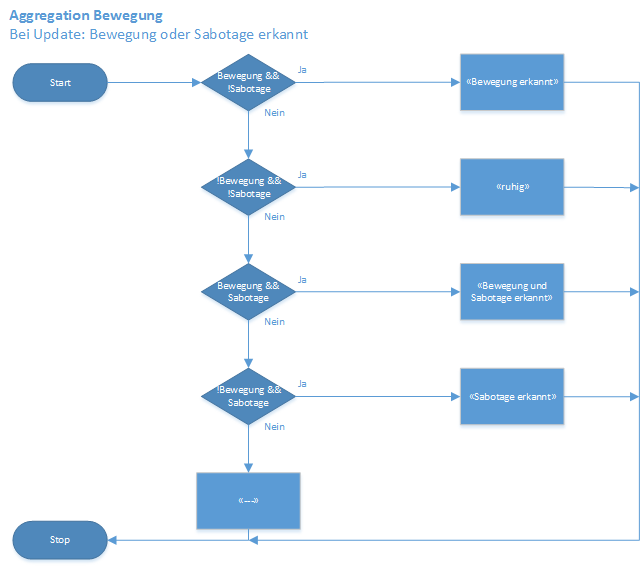
\includegraphics[scale=0.8]{report/img/RuleMotionAggregator}
	\caption{Flowchart Motion Aggregator Rule}
	\label{fig:flowChartMotionAggregator}
\end{figure}

Nachfolgend ist die Definition der Regel in der openhAB DSL beschrieben. Falls keiner der vier möglichen Zustände zutrifft, was nur in einem Fehlerfall möglich ist, wird «---» im Item \lstinline!Motion_Summary! angezeigt.

\begin{lstlisting}[style=csharp, caption=demo.rules - Rule «Motion Aggregator»]
rule "Motion Aggregator"
	when Item Motion_Livingroom received update or
	     Item Motion_Livingroom_Sabotage received update
	then
	if(Motion_Livingroom.state == "true" &&
	   Motion_Livingroom_Sabotage.state == "NO_ERROR") {
		postUpdate(Motion_Summary, "Bewegung erkannt")
	} else if(Motion_Livingroom.state == "false" && 
	          Motion_Livingroom_Sabotage.state == "NO_ERROR") {
		postUpdate(Motion_Summary, "ruhig")	
	} else if(Motion_Livingroom.state == "true" &&
	          Motion_Livingroom_Sabotage.state == "SABOTAGE") {
		postUpdate(Motion_Summary, "Bewegung und Sabotage!")
	} else if(Motion_Livingroom.state == "false" &&
	          Motion_Livingroom_Sabotage.state == "SABOTAGE")  {
		postUpdate(Motion_Summary, "Sabotage")
	} else {
		postUpdate(Motion_Summary, "---")
	}
end
\end{lstlisting}

\pagebreak


\subsection{Deploymentübersicht}

\subsubsection{Binding Azure}
\begin{figure}[H]
	\centering
		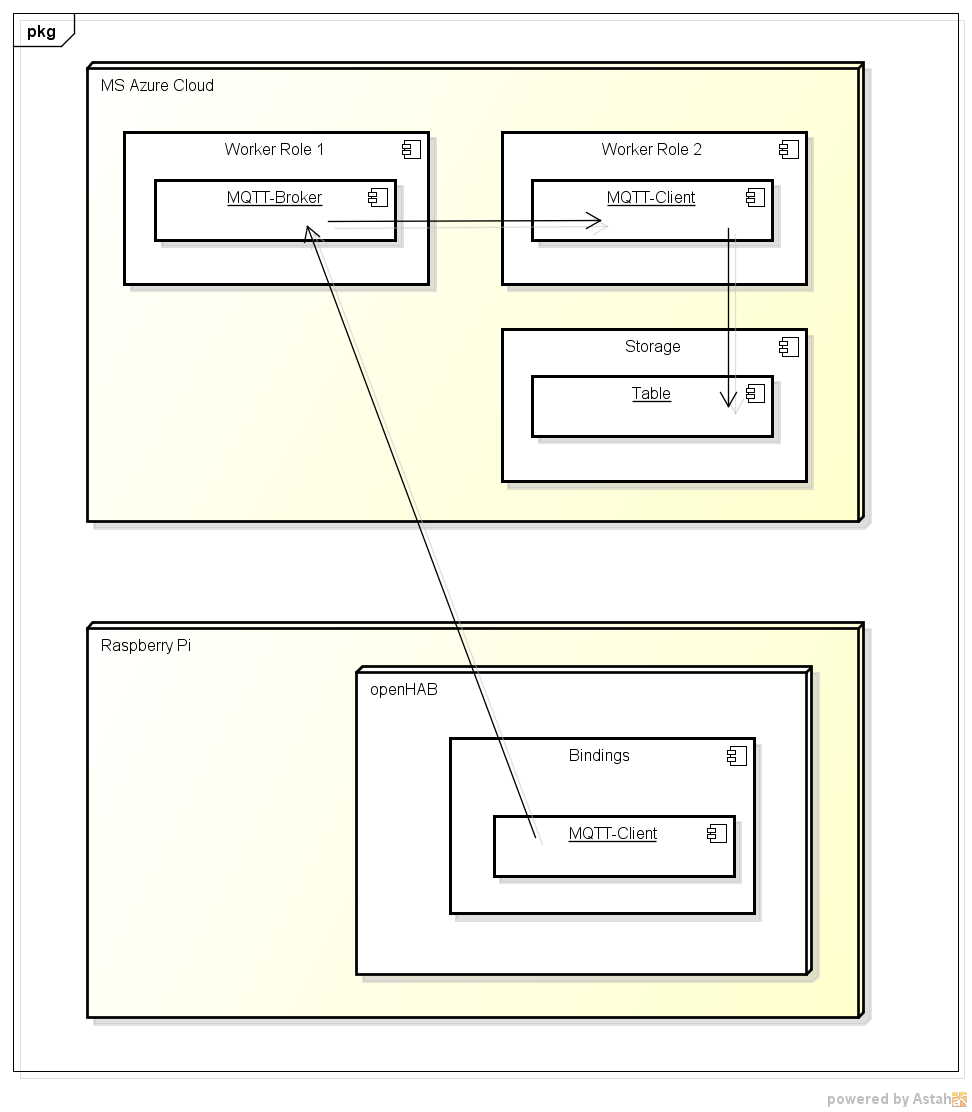
\includegraphics[scale=0.5]{report/img/deployment_binding_azure}
	\caption{Binding Azure Cloud}
	\label{fig:deploymentAzure}
\end{figure}

\subsection{MQTT} \label{sssec:mqtt}
MQTT steht für «Message Queue Telemetry Transport» und ist ein Nachrichten-Protokoll, das speziell für IOT-Anwendungen konzipiert wurde. Es setzt auf dem TCP/IP Stack auf und wird für den Nachrichtenaustausch zwischen verschiedenen, verteilten Maschinen verwendet. \\
Das Protokoll wurde speziell für Systeme designt, die über wenig Speicherplatz und kleiner Netzwerk-Bandbreite verfügen, was bei IOT-Anwendungen meist der Fall ist.

\subsubsection{Funktionsweise}
MQTT folgt dem Prinzip «Publish/Subscribe», sprich Clients können bestimmte Topics abonnieren. Wenn Messages auf dieses Topic gesendet werden, leitet der Broker diese an alle interessierten Clients weiter. \\
In Bezug auf erstellen von Topics agiert der Broker passiv. Das bedeutet, Clients können sich auf beliebigen, selber defnierte, Topics registrieren. Wenn aber niemand auf dieses Topic publiziert, wird der Client nie eine Message erhalten.

\begin{figure}[H]
	\centering
		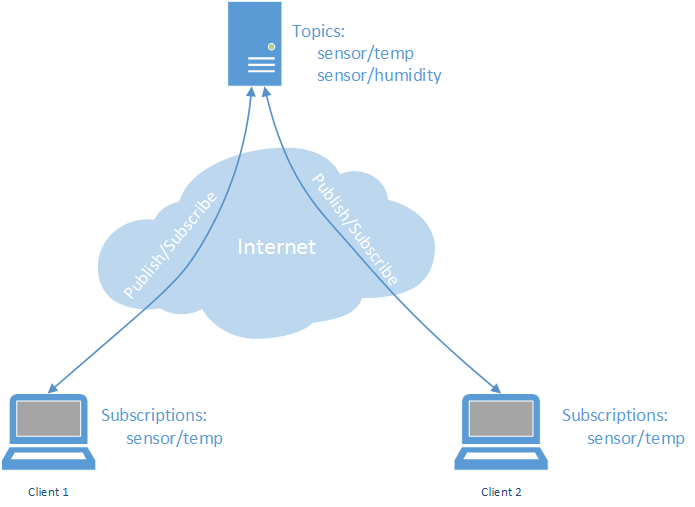
\includegraphics[scale=0.6]{report/img/mqttFunktionsweise}
	\caption{Funktionsweise MQTT}
	\label{fig:funktionsweiseMQTT}
\end{figure}

\subsubsection{Broker}

\textbf{Zertifizierungsstelle/Server-Zertifikat} \\
Da die MQTT-Verbindung verschlüsselt werden soll, müssen verschiedene Zertifikate erstellt werden. Das erstellte Server-Zertifikat muss von einer CA (Certification Authority) signiert werden. Da ein gültiges Zertifikat nicht entgeltlich erworben werden möchte, wird eine eigene Zertifizierungsstelle erstellt. OpenSSl bringt da alle nötigen Mittel für die Erzeugung eines CAs mit. Dies bringt den Nachteil mit, dass Computersysteme diesem Zertifikat nicht automatisch trauen, daher muss dann das Zertifkat von Hand dem Certificate Store als «Trusted Root Certification Authority» hinzugefügt werden. \\

Nachdem die Zertifizierungsstelle erfolgreich generiert wurde, kann das Server Zertifikat erstellt werden. Anschliessend muss dieses Server Zertifikat von der eben erstellten Zertifizierungsstelle signiert werden.

Da sowohl die Zertifizierungsstelle, als auch das Server-Zertifikat auf dem gleichen Computer erstellt werden, muss darauf geachtet werden, dass bei der Erzeugung unterschiedliche Parameter gesetzt werden. Die betroffenen Parameter sind zum Beispiel «Locality Name», «Organizational Name», «Organizational Unit» etc. Falls hier dieselben Werte eingetragen werden, schlägt die Signierung des Serverzertifikates fehl. \\
Weiter muss beachtet werden, dass im Server-Zertifikat der «Common Name» dem FQDN (Fully Qualified Domain Name) des Servers entspricht, auf dem der MQTT-Broker laufen soll. Wird hier beispielsweise nur der Hostname eingetragen, schlägt die Überprüfung des Zertifikates fehl, da sich der CN vom FQDN des Servers unterscheidet.

\textbf{Installation und Konfiguration des Brokers} \\
Wie bereits im Lösugnskonzept erarbeitet, wird als MQTT-Broker «Mosquitto» eingesetzt. Der Broker kann als Binary installiert und über die Commandline gestartet werden.
Nach der Standard-Installation muss der Broker Konfiguriert werden. Dazu wird das File «mosquitto.conf» bearbeitet.
\\Folgende Parameter müssen editiert werden:

\begin{tabularx}{\textwidth}{XX}
		\textbf{Parameter} & \textbf{Erklärung}
		\\ \hline
			bind\_address \\ mqttbrokerba.cloudapp.net &
			IP-Adresse, an den der Default-Listener gebunden wird.
		\\ \hline
			port 8883 &
			Port, auf den der Default-Listener hören soll. Wenn er nicht speziell definiert wird, hört der Listener per Default auf den Port 1883. Da aber mit TLS verschlüsselt wird, muss dieser von Hand auf den dafür vorgesehenen Port 8883 gesetzt werden.
		\\ \hline
			cafile \\ \path{C:\OpenSSL-Win64\bin\m2mqtt_ca.crt} &
			Hier wird der Pfad eingetragen für das zuvor erstellte CA-Zertifikat.
		\\ \hline
			certfile \\ \path{C:\OpenSSL-Win64\bin\m2mqtt_srv.crt\path} &
			Hier wird der Pfad für das PEM-Encodete Server Zertifikat eingetragen.
		\\ \hline
			keyfile \\ \path{C:\OpenSSL-Win64\bin\m2mqtt_srv.key\path} &
			Hier wird der Pfad für das PEM-Encodete Keyfile eingetragen.
		\\ \hline
			tls\_version tlsv1 &
			Diese Option definiert die zu verwendende TLS-Version. Für Openssl (Version 1.0.2) wird tlsv1 verwendet.
		\\ \hline
			password\_file \\ \path{C:\Program Files (x86)\mosquitto\passwords} &
			Das Passwords-File beinhaltet die definierten Benutzernamen und Passwörter, um sich am Broker anzumelden. Durch setzen dieses Pfades wird dies automatisch vom Broker berücksichtigt.
		\\ \hline
\end{tabularx}

Um den Broker zu starten, muss in der Konsole (cmd.exe) in das Installationsverzeichnis (\path{C:\ProgramFiles(x86)\mosquitto\)} navigiert werden. Dort kann der Broker mit der angepassten Konfiguration gestartet werden. Damit in der Konsole Feedback gezeigt wird, wird der Broker im «Verbose-Modus» gestartet: \\
\lstinline!mosquitto -c mosquitto.conf -v! \\

\subsubsection{openHAB MQTT Persistence (Publishing Client)}
\label{sec:mqttPersistenceRealization}
Im Lösungskonzept haben wir bereits erklärt, dass wir die Events auf dem openHAB Eventbus via MQTT an die Cloud übertragen wollen und dass es ein MQTT Plugin für openHAB gibt. Nachdem der Broker installiert wurde wollen wir nun unsere openHAB Items an den Broker senden. Dazu installieren wir das openHAB MQTT Persistence Plugin auf unserem Raspberry Pi: \\
\lstinline!apt-get install openhab-addon-persistence-mqtt!
\\ \\
Danach müssen wir in der openHAB Konfiguration (openhab.cfg) angeben, wie wir uns auf den Broker verbinden wollen:
\begin{lstlisting}[style=csharp, caption=openhab.cfg - MQTT Config]
mqtt:mosquitto.url =  ssl://mqttbrokerba.cloudapp.net:8883
mqtt:mosquitto.user=mosquitto
mqtt:mosquitto.pwd=******************

mqtt-persistence:broker=mosquitto
mqtt-persistence:topic=openhab/items
mqtt-persistence:message={
	"name":"%1$s",
	"state":"%3$s", 
	"date":"%4$s"
}
\end{lstlisting}

Jetzt müssen wir openHAB noch beibringen, wann genau die Items an den Broker gesendet werden sollen. Das geschieht über eine Persistence-Konfiguration. Im Ordner \lstinline!configuration/persistence! erstellen wir ein File namens \lstinline!mqtt.persist! mit dem folgenden Inhalt:

\begin{lstlisting}[style=csharp, caption=mqtt.persist]
Strategies {
	everyMinute : "1 * * * * ?"
	everyHour : "0 0 * * * ?"
	default = everyChange
}

Items {
	* : strategy = everyChange, restoreOnStartup
}
\end{lstlisting}

Damit erreichen wir, dass ein Item immer dann an den Broker gesendet wird, wenn sich der Status des Items ändert. Zudem sollen bei jedem Systemstart alle Items an den Broker geschickt werden. Jetzt fungiert openHAB als ein Publisher.


\subsubsection{Azure Worker Role (Subscribing Client)} \label{sssec:m2mqttClient}
Wie die Abbildung \ref{fig:systemView} auf Seite \pageref{fig:systemView} (Systemübersicht) zeigt, befindet sich nebst dem Broker auch ein Client, in form einer Worker Role, in der Cloud. Die Worker Role abonniert alle Topics und persistiert die Messages im Table bzw. Blob-Storage.

In der \lstinline!OnStart()!-Methode der Worke Role werden zu erst die Referenzen zum Table- und Blob-Storage erzeugt. \\
Danach wird die Verbindung zum MQTT-Broker hergestellt, die Topics definiert, die er abonnieren möchte und der QoS-Level gesetzt. \\
Damit der Client benachrichtigt wird, wenn eine Message eintrifft, wird der Eventhandler \lstinline!client_MqttMsgPublishReceived()! definiert. Die Methode muss die gleichen Parameter entgegennehmen, wie die Delegate-Methode. Das ist einerseits der Sender (Object) und die Event-Argumente. Damit der Eventhandler beim Eintreffen einer Message aufgerufen wird, muss dieser auf dem Event registriert werden: \\ \lstinline!client.MqttMsgPublishReceived += client_MqttMsgPublishReceived;! 

\begin{lstlisting}[style=csharp, caption=WorkerRole.cs - MQTT Topic Subscribe]
public override bool OnStart()
{
  setupStorageConnections();
  MqttClient client = new MqttClient(
            				"mqttbrokerba.cloudapp.net",
               				8883, true, null
               			  );
  client.MqttMsgPublishReceived += client_MqttMsgPublishReceived;
  client.Connect(Guid.NewGuid().ToString(),
  				 "username",
  				 "password"
  				 );
  string[] topics = { "openhab/+" };
  byte[] qos = { MqttMsgBase.QOS_LEVEL_EXACTLY_ONCE };
  client.Subscribe(topics, qos);

  return result;
}
\end{lstlisting}

Im Eventhandler wird dann schlussendlich die Logik zur Persistierung eingefügt. Wenn eine Message über das Topic «openhab/blob» empfangen wird, handelt es sich um eine Fotografie der Webcam. Dieses JPG-File wird als Byte-Array übermittelt und wird so auch im Blob-Storage abgelegt. \\
Bei allen anderen Messages muss es sich um Text handeln, daher werden sie im Table-Storage abgelegt.

\begin{lstlisting}[style=csharp, caption=WorkerRole.cs - EventHandler]
void client_MqttMsgPublishReceived(object sender,
								   		MqttMsgPublishEventArgs e)
{
	if (e.Topic.Equals("openhab/blob"))
	{
		CloudBlockBlob blockBlob = container.
							GetBlockBlobReference(Guid.NewGuid()
								   							.ToString());
		blockBlob.UploadFromByteArray(e.Message,
									  0, e.Message.Length);
    }
	else
	{
    	var message = System.Text.Encoding.
    							  Default.GetString(e.Message);
		Entity entity = new Entity(message);
		TableOperation insertOperation = TableOperation.
											Insert(entity);
		table.Execute(insertOperation);
	}
}
\end{lstlisting}

\textbf{Zertifikat} \\
Da die Verbindung durch SSL/TLS mit einem Self-signed Zertifikat verschlüsselt wird, muss dieses Zertifikat dem Certificate Store des virtuellen Hosts als «Trusted Root Certification Authority» hinzugefügt werden. Dies muss vorgenommen werden, bevor die Worker Role versucht eine Verbindung zum Broker herzustellen. Ansonsten terminiert die Worker Role mit einer Exception, da sie das Zertifikat nicht akzeptiert. \\
Da man zwischen Erzeugung des virtuellen Hosts und dem Start der Worker Role nicht auf die Maschine zugreifen kann, muss das zertifikat programmatisch als Startup-Skript dem Store hinzugefügt werden. Für solche Aufgaben bietet Microsoft Azure die Möglichkeit Startup Tasks zu definieren. Dies wird in der ServiceDefinition vorgenommen, durch einfügen folgender Anweisung:
\begin{lstlisting}[style=csharp, caption=ServiceDefinition.csdef - Startup Task]
<Startup>
	<
		Task commandLine="startup.cmd" executionContext="elevated"
		taskType="simple"
	/>
</Startup>
\end{lstlisting}
Dieser Startup Task führt das Batchfile «startup.cmd» aus, welches das Zertifikat in den Store hinzufügt. Dazu muss das Skript und auch das Zertifikat dem Visual-Studio-Projekt als Element hinzugefügt werden. Für beide Elemente muss in den Eigenschaften der Buildvorgang als «Inhalt» deklariert werden.

\begin{lstlisting}[style=csharp, caption=startup.cmd - Zertifikat hinzufügen]
certutil -addstore root m2mqtt_ca.cer
\end{lstlisting}

Im Sequenzdiagram der Abbildung \ref{fig:sequenzMQTT} wird aufgezeigt, wie die MQTT-Nachrichten nachdem QoS 2 versendet werden.

\begin{figure}[H]
	\centering
		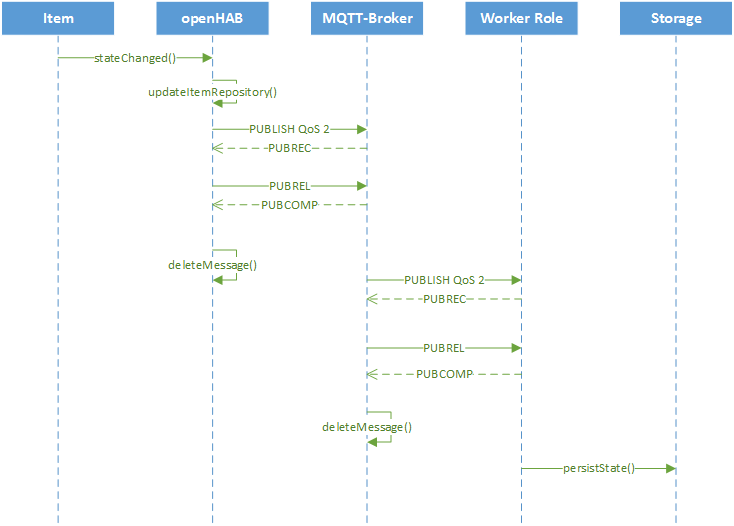
\includegraphics[scale=0.8]{report/img/sequenzDiagramMqtt}
	\caption{Sequenzdiagramm MQTT}
	\label{fig:sequenzMQTT}
\end{figure}


\subsubsection{openHAB MQTT Action}
Normalerweise wird ein openHAB Item direkt via MQTT an die Cloud gesendet, sobald sich der Status des Items ändert. Da unsere Überwachungskamera aber nicht durch ein openHAB Item repräsentiert wird, kann openHAB auch nichts davon an die Cloud schicken. Trotzdem möchten wir gerne einen Snapshot der Kamera an die Cloud senden, sobald der Alarm ausgelöst wurde (siehe Abbildung \ref{fig:sequenceAlarm} - Sequenzdiagramm Alarm auf Seite \pageref{fig:sequenceAlarm} im Lösungskonzept). \\
Deshalb benutzen wir eine sogenannte openHAB Action zum Senden des Snapshots an den MQTT Broker. Die Action kann in der DSL zum beschreiben der Rules ähnlich wie ein statischer Methodenaufruf verwendet werden. Natürlich gibt es diese spezielle Action noch nicht im Standardumfang von openHAB, sondern wir mussten diese in Form eines Action-Plugins selbst programmieren.

\textbf{Programmierung der MQTT Action}\\
Zum Entwickeln von openHAB Plugins muss eine entsprechende Eclipse Umgebung eingerichtet werden. Dies sollte sich noch als der schwierigste Teil davon herausstellen. Eine Anleitung dazu findet man unter \url{https://github.com/openhab/openhab/wiki/IDE-Setup}. Bei uns hat nur die Variante mit «yoxos» funktioniert. Und auch bei dieser Anleitung mussten wir einige Tricks anwenden. Bei Schritt 8) musste die JDK Version in den Projekteinstellungen zunächst auf 1.6 zurückgestuft werden und vor Schritt 9) wieder auf Version 1.7. Beim Kompilieren werden alle openHAB Artifakte erstellt: OpenHAB selbst, alle Bindings, Actions und sonstige Plugins, sowie auch die Eclipse RCP's des openHAB Designers für alle Zielsysteme. 
\\ \\
Sobald Eclipse vollständig eingericht wurde kann ein Action Skeleton anhand eines Maven Archetypes generiert werden. Eine Anleitung dazu befindet sich im openHAB GitHub Wiki: \url{https://github.com/openhab/openhab/wiki/How-To-Implement-An-Action}. \\
Die openHAB Runtime wird die Action-Aufrufe in den Rules später zur Laufzeit an die statischen Java-Methoden im Action-Plugin binden. Damit das später alles sauber funktioniert und auch die Dependency Injection von gewissen Service-Objekten gemacht werden kann müssen die Dateien OSGI-INF/action.xml und META-INF/MANIFEST.MF angepasst werden:

\begin{lstlisting}[style=csharp, caption=OSGI-INF/action.xml]
<?xml version="1.0" encoding="UTF-8"?>

<scr:component xmlns:scr="http://www.osgi.org/xmlns/scr/v1.1.0"
     activate="activate" deactivate="deactivate" immediate="true"
     name="org.openhab.action.mqtt.action">
	<implementation class="org.openhab.action
		.mqtt.internal.MqttActionService" />
	<service>
		<provide interface="org.openhab.core
			.scriptengine.action.ActionService" />
		<provide interface="org.osgi.service
			.cm.ManagedService" />
	</service>
	<property name="service.pid" type="String" 
		value="org.openhab.mqtt-action" />
	<reference bind="setMqttService" cardinality="1..1"
	     interface="org.openhab.io
	     	.transport.mqtt.MqttService" name="MqttService"
	     policy="static" unbind="unsetMqttService"/>	
</scr:component>

\end{lstlisting}

\begin{lstlisting}[style=csharp, caption=META-INF/MANIFEST.MF]
Manifest-Version: 1.0
Private-Package: org.openhab.action.mqtt.internal
Ignore-Package: org.openhab.action.mqtt.internal
Bundle-License: http://www.eclipse.org/legal/epl-v10.html
Bundle-Name: openHAB Mqtt Action
Bundle-SymbolicName: org.openhab.action.mqtt
Bundle-Vendor: openHAB.org
Bundle-Version: 1.7.0.qualifier
Bundle-Activator: org.openhab.action.mqtt.internal.MqttActivator
Bundle-ManifestVersion: 2
Bundle-Description: This is the Mqtt action of the open Home Aut
 omation Bus (openHAB)
Import-Package: org.apache.commons.lang,
 org.openhab.core.scriptengine.action,
 org.openhab.io.transport.mqtt,
 org.osgi.framework,
 org.osgi.service.cm,
 org.slf4j
Bundle-DocURL: http://www.openhab.org
Bundle-RequiredExecutionEnvironment: JavaSE-1.6
Service-Component: OSGI-INF/action.xml
Bundle-ClassPath: .
Bundle-ActivationPolicy: lazy

\end{lstlisting}

Dank diesen Konfigurationen wird der gleiche MQTT-Service Injected, der auch im MQTT-Persistence Plugin eingesetzt wird und die statischen Java Methoden aus der Klasse org.openhab.action.mqtt.internal.Mqtt werden für die DSL sichtbar. Zudem stellt die openHAB Runtime der MQTT Action die zugehörigen Konfigurationen zur Verfügung, die in der globalen Konfigurationsdatei hinterlegt wurden (openhab.cfg).\\ \\

\textbf{Installation MQTT Action}\\
Nachdem wir die MQTT Action programmiert hatten, mussten wir sie mit Hilfe von Eclipse als .jar Datei exportieren. Danach haben wir in der Konfigurationsdatei von openHAB (openhab.cfg) den Eintrag für die MQTT Action gemacht. Diese verweist auf den selben Broker, den wir auch für das Persitence Plugin benötigen.


\begin{lstlisting}[style=csharp, caption=openhab.cfg]
mqtt-action:broker=mosquitto
\end{lstlisting}

Anschliessend haben wir die .jar Datei ins Add-on Verzeichnis unserer openHAB Installation kopiert. Die openHAB Runtime erkennt das neue OSGI-Modul sofort und aktiviert es.

\textbf{Verwendung der MQTT Action}\\
Die MQTT Action implementiert zwei Methoden: sendMQTTString(topic, message) und sendMQTTFile(topic, fileUrl). Die erste Methode sendet einen String an das Topic des vorkonfigurierten Brokers. Die zweite Methode ist diejenige, weswegen wir das Plugin überhaupt entwickelt haben. Sie nimmt eine URL entgegen, lädt den Inhalt von dort herunter und sendet ihn an das gewünschte Topic des Brokers. Beide Methoden können von jetzt an in openHAB Rules oder Scripts verwendet werden.

\subsection{Android App}
Im Lösungskonzept in Abschnitt \ref{sec:androidArchSolution} ab Seite \pageref{sec:androidArchSolution} haben wir bereits erklärt, wie die Architektur der App aussieht. In diesem Abschnitt gehen wir auf die eingesetzten Frameworks, wichtige Klassen und das User Interface Design ein.

\subsubsection{Frameworks und Libraries}
Für Android gibt es mittlerweile eine grosse Vielzahl an äusserst hilfreichen und robusten Frameworks und Libraries, die den Entwickleralltag enorm erleichtern. Manche der Frameworks haben einen starken Einfluss darauf, wie der Code strukturiert wird. Für das Verständnis des Codes ist es deshalb wichtig, sich mit ReactiveX, Retrofit und Butterknife vertraut zu machen. Folgende Liste beinhaltet alle Gradle Build Dependencies:

\begin{itemize}
	\item \lstinline!com.squareup.retrofit:retrofit:1.9.0!
    \item \lstinline!io.reactivex:rxandroid:0.24.0!
    \item \lstinline!com.android.support:appcompat-v7:22.0.+!
    \item \lstinline!com.android.support:cardview-v7:21.0.+!
    \item \lstinline!com.android.support:recyclerview-v7:21.0.+!
    \item \lstinline!com.squareup.okhttp:okhttp:2.4.0-RC1!
    \item \lstinline!com.rengwuxian.materialedittext:library:2.0.3!
    \item \lstinline!com.jakewharton:butterknife:6.1.0!
    \item \lstinline!jp.wasabeef:recyclerview-animators:1.2.0@aar!
    \item \lstinline!com.nispok:snackbar:2.10.+!
    \item \lstinline!com.github.clans:fab:1.5.0!
    \item \lstinline!com.google.android.gms:play-services:6.5.87!
\end{itemize}


\textbf{ReactiveX} \\
Die Reactive Extension wurde usprünglich für .NET entwickelt und ist mittlerweile fester Bestandteil davon. Heute gibt es die Library auch für diverse andere Plattformen, darunter Java bzw. auch eine spezielle Version für Android. ReactiveX verwendet das Programmierparadigma der reaktiven Programmierung und unterstützt den Programmierer beim Ausdrücken von komplizierten Datenflüssen. In der konventionellen, imperativen Programmierung herrscht das Pull-prinzip, sodass Änderungen an Daten aktiv geholt werden müssen. ReactiveX hingegen «pusht» neue Daten in die Konsumenten hinein. Dabei berücksichtigt ReactiveX auch viele Concurrency-aspekte automatisch.\\

Das Folgende (leicht vereinfachte) Beispiel stammt aus unserer App und demonstriert sehr gut die Vorteile von ReactiveX. Von der openHAB REST API soll ein Item geladen werden, danach soll der boolsche Wert invertiert und wieder an die API zurückgesendet werden. Bevor der neue Status im User Interface angezeigt wird, wird der Status aus Konsistenzgründen noch einmal geladen:
\pagebreak
\begin{lstlisting}[style=csharp, label={lst:reactiveXSample}, caption=ReactiveX Beispiel]
api.getItem("Alarm_active")
.flatMap(item -> {
	 return Observable.just(item.state.equals("ON") ? "OFF" : "ON")
})
.flatMap(state -> api.sendCommand("Alarm_active", state))
.flatMap(aVoid -> api.getItem("Alarm_active"))
.subscribeOn(Schedulers.io())
.observeOn(AndroidSchedulers.mainThread())
.subscribe(item-> {
	updateUi(item.state);
});
\end{lstlisting}

Jede dieser aneinander gereihten Methoden gibt ein Objekt von Typ \lstinline!Observable<T>! zurück und modifiziert das vorherige Observable. Der Code in den Lambdas wird aber noch nicht ausgeführt sondern lediglich als Callable im Observable hinterlegt, für den Zeitpunkt wo Daten «hindurchfliessen». Erst beim Aufruf von \lstinline!subscribe()! auf Zeile 9 wird die Maschine in Gang gesetzt. Die beiden Methoden auf Zeile 7 und 8 sind dazu gedacht, dass die API Calls in einem Hintergrundthread und das letzte Resultat wieder im Android Mainthread ausgeführt werden. \\
Ohne ReactiveX müsste man für diese Aufgabe drei Callback-Handler registrieren, die dann jeweils den nächsten API Call anstossen. Deshalb haben wir ReactiveX so oft wie möglich verwendet, mit Ausnahme von einigen Spezialfällen. 

\textbf{Retrofit} \\
Diese Library erleichtert das Konsumieren von REST Webservices. Man erstellt zunächst ein Java Interface und schreibt die Methodensignaturen für die Requests. Der Rückgabetyp ist entweder das erwartete POJO oder \lstinline!void!. Methoden mit dem Rückgabetyp \lstinline!void! werden automatisch asynchron ausgeführt, verlangen aber einen Callback Handler als zusätzlichen Parameter. Methoden mit POJO Rückgabetypen werden synchron ausgeführt. Danach müssen alle Methoden noch mit den Annotations von Retrofit versehen werden. Unter anderem werden die gewünschte HTTP Methode (\lstinline!GET, PUT, POST, DELETE,! \ldots), ein relativer URL Pfad und die Parameter angegeben. Besonders komfortabel ist, dass das Interface nicht selbst implementiert werden muss. Retrofit generiert die entsprechende Klasse anhand der Annotations. Das Erzeugen einer Instanz ist denkbar einfach:

\begin{lstlisting}[style=csharp, label=lst:retrofitCreation, caption=Retrofit - Service-Klasse generieren]
RestAdapter adapter = new RestAdapter.Builder()
	.setEndpoint(endpoint)
	.setConverter(new GsonConverter(gson))
	.build();
	
OpenHabApi api = adapter.create(OpenHabApi.class);
\end{lstlisting}

In Listing \ref{lst:retrofitCreation} auf Zeile 3 wird ein \lstinline!GsonConverter! übergeben. Dieser sorgt dafür, dass die JSON Response korrekt deserialisiert und auf den gewünschten POJO Typ gemappt wird. Dem \lstinline!gson!-Objekt selbst können noch sogenannte TypeAdapter hinzugefügt werden, um mehr Kontrolle beim Mapping zu haben.\\
\\ 
Noch besser als das automatische Generieren der Service-Klassen ist an Retrofit der Support für ReactiveX. Wenn man asynchrone REST Calls machen möchte, würde man normalerweise einen Callback Handler übergeben, wie bereits beschrieben. Es gibt allerdings eine elegantere Variante. Sofern ReactiveX als Dependency im Projekt aufgelöst werden kann, ist es möglich, den Rückgabetyp der Methoden im Service-Interface mit \lstinline!Observable<T>! zu deklarieren. Anschliessend weiss Retrofit, dass die Methode asynchron und mit Hilfe von ReactiveX ausgeführt werden soll. Beim Aufruf der Methode erhält man also nicht direkt das POJO, sondern ein Observable, welches man subscriben kann. Sobald sich ein Subscriber anmeldet wird der Request ausgeführt und das Resultat an den Subscriber geschickt. Folgendes Service-Interface deklariert die Methoden, welche bereits aus dem ReactiveX Code-Beispiel in Listing \ref{lst:reactiveXSample} bekannt sind:

\begin{lstlisting}[style=csharp, label=lst:retrofitInterface, caption=OpenHabApi Service-Interface]
public interface OpenHabApi {
	@GET("/rest/items/{item}?type=json")
	Observable<Item> getItem(@Path("item") String item);
    
	@Headers("Content-type: text/plain")
	@POST("/rest/items/{item}")
	Observable<Void> sendCommand(@Path("item") String item, 
		@Body TypedInput command
	);
}
\end{lstlisting}

Dank dem Zusammenspiel von ReactiveX und Retrofit wird dem Programmierer ein gewaltiger Teil an Fleissarbeit abgenommen. Es kann schneller entwickelt werden, die möglichen Fehlerquellen werden reduziert und die Lesbarkeit bzw. Nachvollziehbarkeit verbessert sich.


\textbf{Butterknife} \\
Butterknife ist eine nützliche kleine Library zur Dependency Injection von View Komponenten in Activities. Jede Activity besitzt in der Regel eine Root-View, die in einem Layout Resource File mit XML definiert wird. In diesen Layout Files befinden sich typischerweise weitere User Interface Elemente, wie Buttons, Input-Felder oder Bilder. Die Activity ist dazu gedacht, jene Elemente mit Code zu beleben, also Events zu behandeln, Texte zu aktualisieren und so weiter. Die Referenzen auf diese Elemente muss sich die Activity selbst beschaffen, indem sie die \lstinline!findViewById(int id)! Methode aufruft und das Element anschliessend einer lokalen- oder Instanzvariablen zuweist. Die Methode \lstinline!findViewById(int id)! hat den Rückgabetyp \lstinline!View!, deshalb müssen alle Element explizit gecastet werden.\\

Butterknife macht diese Tipparbeit überflüssig, indem die Elemente als Instanzvariablen deklariert und mit einer Annotation versehen werden:

\begin{lstlisting}[style=csharp, label=lst:butterknifeSample1, caption=Butterknife Beispiel 1]
public class SampleActivity extends Activity {

	@InjectView(R.id.button)
	Button mButton;
	
	@Override
	protected void onCreate(Bundle savedInstanceState) {
		super.onCreate(savedInstanceState);
		setContentView(R.layout.activity_sample);
		ButterKnife.inject(this);
		// instead of: mButton = (Button) findViewById(R.id.Button);
	}
}
\end{lstlisting}

Ein Vorteil ergibt sich vorallem bei Activities mit vielen referenzierten User Interface Elementen. Butterknife erleichtert zudem das Behandeln von Events, indem Methoden ebenfalls mit einer Annotation versehen werden, anstatt dass die Activity ein Callback Interface implementieren muss bzw. anonyme Klassen verwendet werden:

\begin{lstlisting}[style=csharp, label=lst:butterknifeSample2, caption=Butterknife Beispiel 2]
@OnClick(R.id.button)
public void onClickButton(View view) {
	// do something useful
}
\end{lstlisting}



\subsubsection{Wichtige Klassen}
\label{sec:importantClasses}
Zum besseren Verständnis werden hier einige ausgewählte Klassen und Packages genauer erklärt.

\textbf{ch.hsr.baiot.openhab.sdk.model.*}\\
Dieses Package ist Teil des SDK und beinhaltet die POJO Model-Klassen sowie einige Hilfsklassen. Die JSON Responses der REST API werden auf diese Model-Klassen gemappt. Manche Model-Klassen implementieren das von uns definierte Interface \lstinline!MemberEquals! mit der Methode \lstinline!hasEqualMembers(other)!. Grund dafür ist, dass die Methode \lstinline!equals(other)! bereits überschrieben wird und die Gleichheit zweier Objekte nur anhand des jeweiligen «Primärschlüssels» festgestellt wird. In einigen Fällen soll aber auch überprüft werden können, ob alle Instanzvariablen gleich sind, beispielsweise um zu bemerken, ob ein Objekt sich nach dem erneuten Laden verändert hat.

\begin{lstlisting}[style=csharp, label=lst:modelSample, caption=Item.java - Beispiel einer Model-Klasse]
package ch.hsr.baiot.openhab.sdk.model;

[...] // Imports

public class Item implements MemberEquals<Item>{
	public String type  = "";
	public String name = "";
	public String state = "";
	public String link = "";

	@Override
	public boolean equals(Object o) {
		if (this == o) return true;
		if (o == null || getClass() != o.getClass()) return false;
		Item item = (Item) o;
		if (!name.equals(item.name)) return false;
		return true;
	}

	@Override
	public int hashCode() { return name.hashCode();}

	@Override
	public boolean hasEqualMembers(Item other) {
		if(this == other) return true;
		if(other == null) return false;

		if(this.type != null ? !this.type.equals(other.type) : 
			other.type != null) return false;
		if(this.state != null ? !this.state.equals(other.state) : 
			other.state != null) return false;
		if(this.link != null ? !this.link.equals(other.link) : 
			other.link != null) return false;
		return true;
	}
}
\end{lstlisting}

\textbf{ch.hsr.baiot.openhab.sdk.model.WidgetListModel}\\
OpenHAB Sitemaps definieren eine baumartige Stuktur aus Pages und Widgets. Jede Page besteht aus einer Collection von Widgets. Widgets können weitere Pages referenzieren. In der App wird immer jeweils eine Page angezeigt, die durch HTTP Long-Polling oder manuelles Laden oft aktualisiert wird. Die Klasse \lstinline!WidgetListModel! hat eine Setter-Methode für eine Liste von Widgets. Danach stellt die Klasse fest, ob Widgets innerhalb der Liste hinzugefügt, entfernt, verschoben oder sonst inhaltlich verändert wurden. Die Änderungen werden danach jeweils in Form eines \lstinline!ListModificationEvent! auf einem ReactiveX Observable emittiert. User Interface Elemente (z.B. \lstinline!RecyclerView! bzw. \lstinline!RecyclerView.Adapter!) können dann auf dieses Observable subscriben und werden aktiv über Modifikationen an der Liste benachrichtigt, ohne dass das User Interface Element etwas über den Reload wissen muss. Für das User Interface unterscheidet sich dieses Design nur geringfügig vom klassischen Observer-Pattern. 

\begin{lstlisting}[style=csharp, label=lst:widgetListModel, caption=Auszug aus WidgetListModel.java]
package ch.hsr.baiot.openhab.sdk.model;

[...] // Imports

public class WidgetListModel {
	
	[...] // Instance variables, getters

	public void setWidgets(List<Widget> modified) {

		List<Widget> original = new ArrayList<>(widgets);
		List<Widget> state = new ArrayList<>(widgets);

		List<Widget> changed = ListUtils.changed(original, modified);
		notifyChanged(changed, original);
		state = ListUtils.update(state, changed);

		[...] // Detect removed, added, moves
		
		widgets = modified;
	}

	public void notifyChanged(List<Widget> changed, 
							 List<Widget> original) {
		for(Widget widget : changed) {
			int index = original.indexOf(widget);
			subject.onNext( new ListModificationEvent<Widget>(
					widget,
					ListModificationEvent.CHANGED,
					index,
					index
			));
		}
	}

	[...] // notifyRemoved, notifyAdded, getMoves

	public Observable<ListModificationEvent<Widget>>
	onModification() {
		return subject;
	}
}

\end{lstlisting}

\textbf{ch.hsr.baiot.openhab.app.adapter.WidgetListAdapter}\\
Diese Klasse erbt vom Typ \lstinline!RecyclerView.Adapter! und verbindet eine Collection von Widgets mit einer \lstinline!RecyclerView!. Die RecyclerView fragt den Adapter nach der Anzahl von Elementen, lässt die Elemente erzeugen und sagt dem Adapter, dass er ein Element an das jeweilige Pendent in der Liste binden soll. Wenn sich die Liste im Adapter ändert, kann dar Adapter der RecyclerView mitteilen, inwiefern sich die Liste verändert hat. Die RecylcerView fragt den Adapter danach wieder entsprechend ab. Dieses Pattern wird in vielen User Interface Frameworks zum Anzeigen von Listen verwendet, so auch in Android. Die Klasse \lstinline!WidgetListAdapter! ist ein Subscriber des \lstinline!WidgetListModel!, wie bereits im Abschnitt zuvor beschrieben. Jedoch kennt der Adapter das ListModel nicht direkt, sondern betrachtet dieses nur als ReactiveX Observable.

\begin{figure}[H]
	\centering
		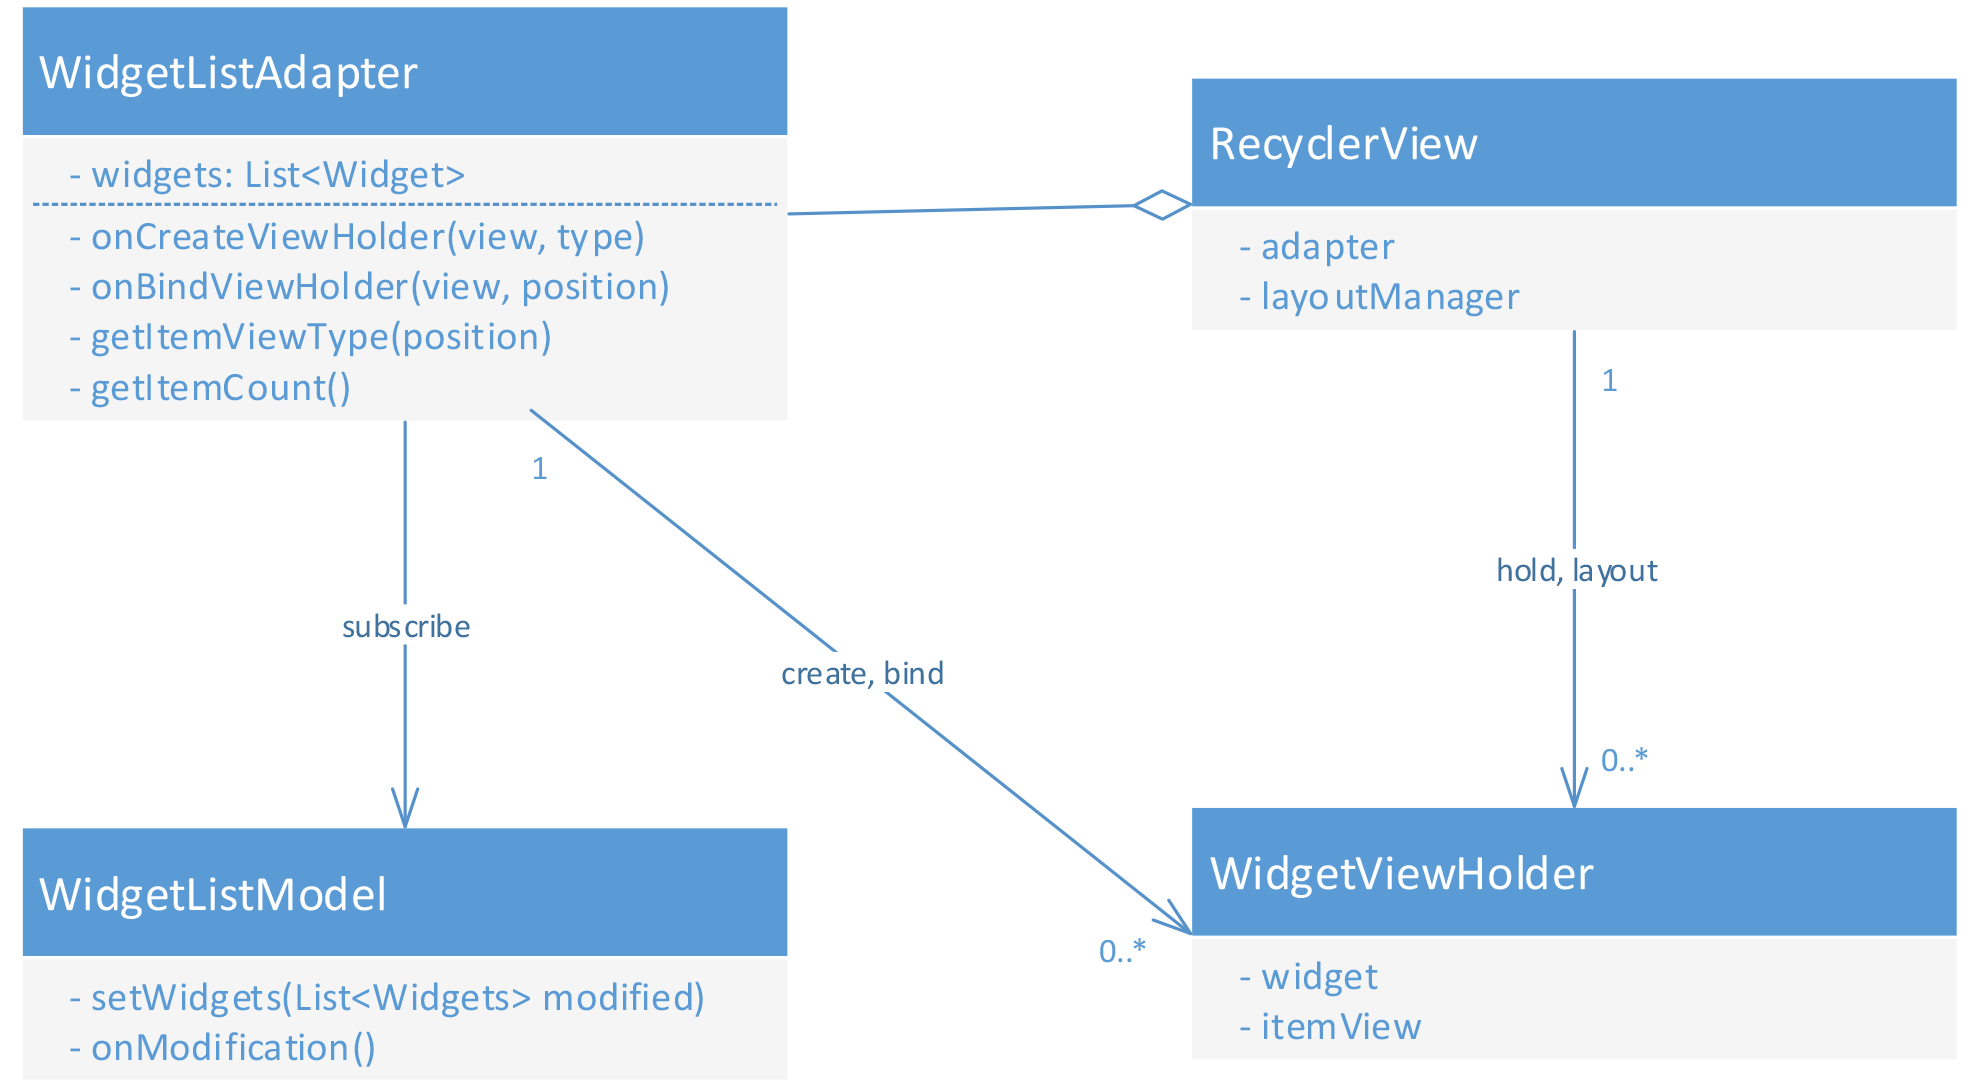
\includegraphics[width=\textwidth]{report/img/recycler_view.png}
	\caption{Klassendiagramm WidgetListAdapter mit Collaborators}
	\label{fig:recylerViewClasses}
\end{figure}

\textbf{ch.hsr.baiot.openhab.app.widget.*}\\
Die User Interface Elemente, die in der RecyclerView als Listeneinträge dargestellt werden, haben pro «Typ» jeweils ein eigenes XML Layout Resource File. Das Layout wird danach vom Android OS instanziiert und einem sogenannten \lstinline!ViewHolder! zugewiesen. ViewHolder sind jene Objekte, die zwischen RecyclerView und Adapter ausgetauscht werden (siehe Abbildung \ref{fig:recylerViewClasses}). ViewHolder Objekte referenzieren die Layoutinstanz und werden im Adapter erzeugt. Das Einsetzen der Daten geschieht auf Anfrage der RecyclerView im Adapter und nennt man «Binding». Im Package \lstinline!ch.hsr.baiot.openhab.app.widget! befinden sich Subklassen von ViewHolder (\lstinline!Widget*.java!). Die Subklassen werden benötigt, damit unterschiedliche Arten von Listeneinträgen in der RecyclerView dargestellt werden können. Beispielsweise solche mit Icon und Text, Detailtext oder solche mit einem Schalter und so weiter. 

\begin{lstlisting}[style=csharp, label=lst:widgetLayoutSample, caption={Layout mit Icon, Text und Detailtext}]
<?xml version="1.0" encoding="utf-8"?>
<RelativeLayout
	xmlns:android="http://schemas.android.com/apk/res/android"
	android:layout_width="match_parent"
	android:layout_height="72dp">

	<LinearLayout
		android:orientation="vertical"
		android:layout_marginTop="16dp"
		android:layout_marginLeft="72dp"
		android:layout_width="match_parent"
		android:layout_height="wrap_content">

		<TextView
			android:id="@+id/text_view"
			android:fontFamily="sans-serif-medium"
			android:textColor="#000000"
			android:textSize="16sp"
			android:layout_width="match_parent"
			android:layout_height="wrap_content" />

		<TextView
			android:id="@+id/text_detail"
			android:fontFamily="sans-serif"
			android:textColor="#000000"
			android:textSize="14sp"
			android:layout_width="match_parent"
			android:layout_height="wrap_content" />

	</LinearLayout>

	<ImageView
		android:id="@+id/icon"
		android:src="@drawable/icon_dummy"
		android:layout_marginLeft="16dp"
		android:layout_marginTop="16dp"
		android:layout_width="40dp"
		android:layout_height="40dp" />
</RelativeLayout>
\end{lstlisting}

\textbf{ch.hsr.baiot.openhab.app.activity.PageActivity}\\
Die wichtigste Activity in unserer App ist die \lstinline!PageActivity!. Sie stellt jeweils eine Page einer Sitemap dar. Für jede Hierarchiestufe in der Sitemap kommt eine neue PageActivity auf den Android Activity Stack. Die PageActivity besitzt unter anderem eine \lstinline!RecyclerView!, einen \lstinline!WidgetListAdapter! und ein \lstinline!WidgetListModel!. Mit Hilfe der Klassen aus dem SDK wird die Page via REST API geladen und die Widgets der Page an das WidgetListModel übergeben. Das WidgetListModel erkennt die Veränderung an der Liste von Widgets (zu Beginn war diese leer) und benachrichtigt die Subscriber über die Veränderungen. Der WidgetListAdapter ist solch ein Subscriber, wodurch die Widgets letztlich in die RecyclerView gelangen. Die PageActivity koordiniert also das Zusammenspiel dieser Komponenten. Das mag etwas komplex erscheinen, jedoch ist somit eine hohe Kohäsion und eine geringe Kopplung erreicht und der Code in den einzelnen Klassen ist leicht nachzuvollziehen. In der offiziellen openHAB App für Android sieht man was passiert, wenn versucht wird die gleiche Aufgabe mit nur einer Klasse zu lösen. Das Ergebnis ist eine gigantische Klasse mit Methoden, die zweihundert Zeilen gerne überschreiten.\\ \\
Wie schon erwähnt lädt die PageActivity initial die gewünschte Page. Anschliessend soll der openHAB Server die App informieren, sobald sich etwas auf dieser Page verändert hat. Dazu verwendet die PageActivity den \lstinline!LongPollingSocketClient! aus unserem SDK. Durch einen Bug von openHAB ist die Response des Long-Polling Requests oftmals leer, sodass die Page konventionell aktualisiert werden muss. Wenn der Long-Polling Request ein Timeout überschreitet, ohne eine Response erhalten zu haben, passiert dasselbe.

\begin{figure}[H]
	\centering
		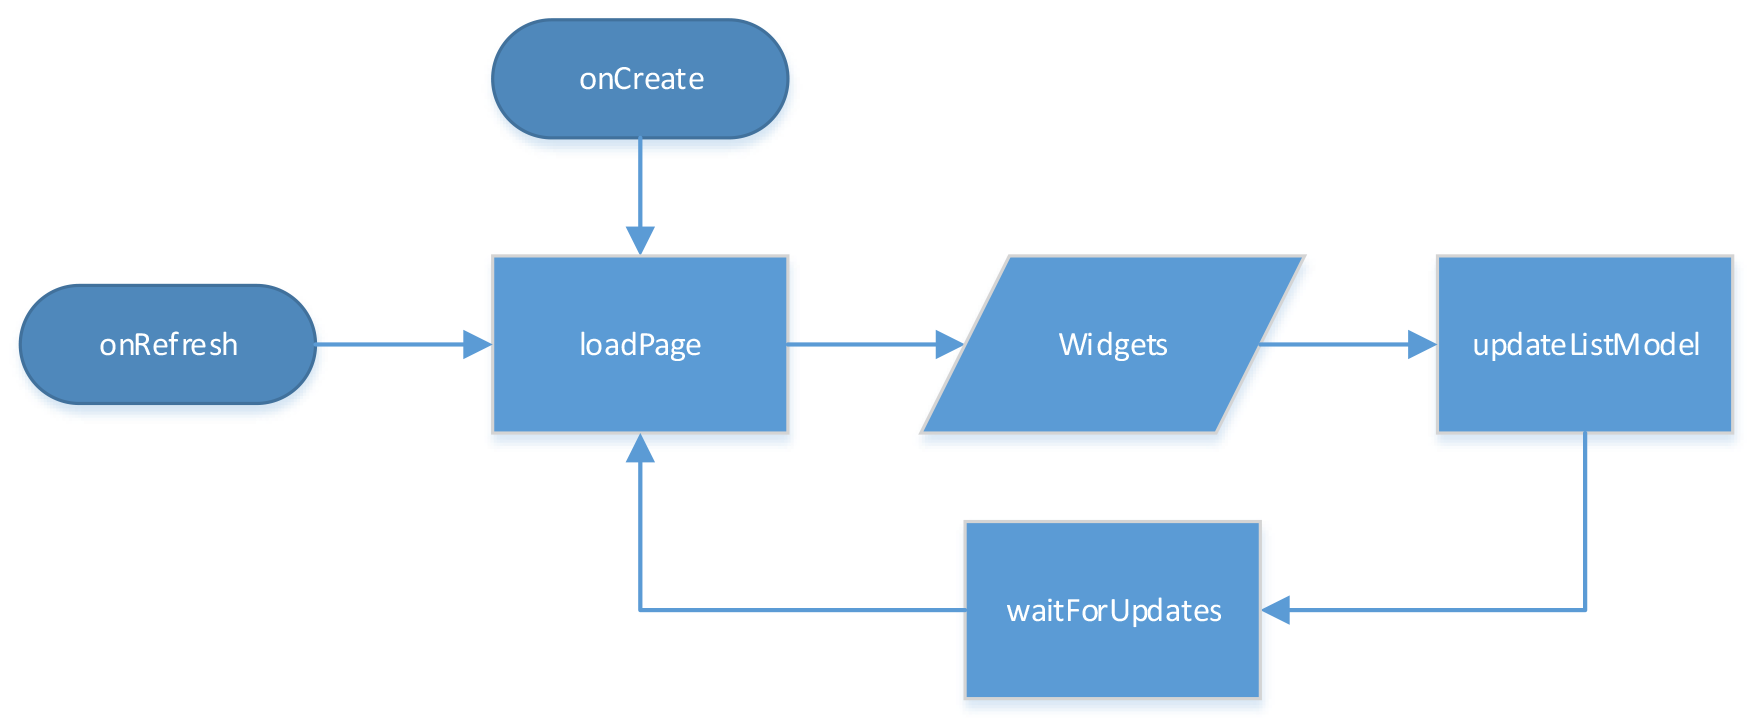
\includegraphics[width=\textwidth]{report/img/page_activity.png}
	\caption{PageActivity Ablauf (vereinfacht dargestellt)}
	\label{fig:pageActivityWorkflow}
\end{figure}

In Abbildung \ref{fig:pageActivityWorkflow} wird der Ablauf beim Laden anhand eines Flussdiagramms vereinfacht aufgezeigt. In dieser Darstellung ist nicht ersichtlich, wie die PageActivity den Ablauf bei Fehlern oder beim Pausieren (im Sinne des Android Activity Lifecycle) unterbricht.

\subsubsection{Material Design}

\subsection{Push-Notifications}
\label{sec:notificationRealization}
Der Mobile-Client wird durch Push-Notifications benachrichtig, sobald der Alarm ausgelöst wird. Umgesetzt wird dies mithilfe des Google Cloud Messaging Dienstes.

\subsubsection{Cloud}
Um den GCM-Dienst nutzen zu können, muss zu erst in der Google Developer Console (\url{https://console.developers.google.com}) ein Projekt erstellt werden mit einer Cloud-Messaging-API. Für diese API kann ein Schlüssel erzeugt werden, der für das Versenden der Notification über die neu erstellte API benötigt wird.

Ausgelöst wird der ganze Vorgang durch die MQTT-Nachricht «alarm\_activated». Die Worker Role nimmt diese Nachricht entgegen und erzeugt eine Notification-Message:

\begin{lstlisting}[style=csharp, caption=Notification.cs - Notification Message]
{
  "registration_ids" : ["APA91bHun4MxP5egoKMwt2KZFBaFUH-1RYqx..."],
  "data" : {
  	"message" : "Alarm wurde ausgeloest!"
  }
}
\end{lstlisting}

Die Registration-Id bezeichnet den Client, der die Message erhalten soll. Dazu müssen sich die Clients zuvor bei GCM registrieren und erhalten dann die Id. Diese Message muss also für jeden Client einzeln über einen HTTP-Post gesendet werden. GCM weiss anhand des Id-Strings an welche Android-Clients er die Message weiterleiten soll.

Folgende Grafik stellt den Registrations-Vorgang dar:
\begin{figure}[H]
	\centering
		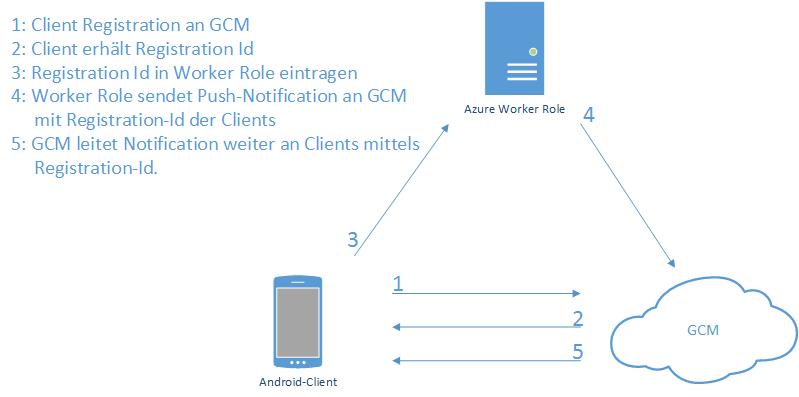
\includegraphics[scale=0.7]{report/img/gcm}
	\caption{Vorgang Push-Notification}
	\label{fig:notification}
\end{figure}

Die nachfolgende Grafik (Abbildung \ref{fig:sequenzNotification}) zeigt auf, wie anhand der MQTT-Message die Notification ausgelöst wird. OpenHAB bemerkt eine Statusänderung eines Items und weiss anhand der Persistency Konfiguration, dass das Item via MQTT an den Broker geschickt werden soll (näheres dazu im Abschnitt \ref{sec:mqttPersistenceRealization} auf Seite \pageref{sec:mqttPersistenceRealization}). Die Worker Role empfängt die Message und entscheidet aufgrund deren Inhalt, ob eine Notification gesendet werden muss. Sollte dies der Fall sein, wird eine Push-Notification beim GCM-Dienst ausgelöst.

\begin{figure}[H]
	\centering
		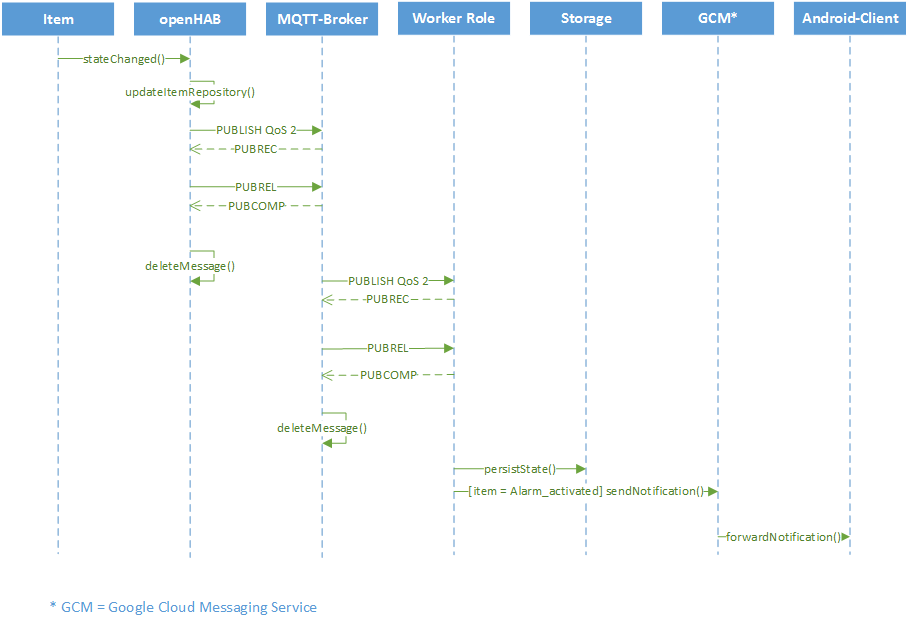
\includegraphics[scale=0.65]{report/img/sequenzDiagramNotification}
	\caption{Sequenzdiagramm MQTT-Notification}
	\label{fig:sequenzNotification}
\end{figure}

\subsubsection{Android-Client}
Wie bereits erklärt benötigt die Worker Role eine Registration-Id um das Android Phone referenzieren zu können. Die Registration-Id ist an ein GCM Projekt gekoppelt und wird in der Android App mit Hilfe des Google PlayServices SDK beim GCM-Dienst angefordert. Die Registration-Id muss dann in eigener Verantwortung an die Worker Role übertragen und geheim gehalten werden. Um eine Nachricht zu erhalten muss ein Android BroadcastReceiver im App-Projekt vorhanden sein, der die Nachricht entgegennimmt und zur Verarbeitung an einen IntentService weitergibt. Dort wird das Notification UI-Element (Dialog am oberen Bildschirmrand) erzeugt und angezeigt.

\subsection{Sicherheit}
Aus technischer Sicht können folgende Massnahmen getroffen werden, um die im Lösungskonzept beschriebenen Schwachstellen zu sichern:
\begin{itemize}
	\item Verschlüsselung der MQTT-Verbindung.
	\item Anmeldung am MQTT-Broker durch Benutzername \& Passwort.
	\item Verschlüsselung des WLANs.
\end{itemize}

\subsubsection{Verschlüsselung MQTT-Verbindung}
Die Verbindung zum MQTT-Broker wird durch SSL/TLS Verschlüsselt. Dazu wird ein Self-signed Zertifikat eingesetzt. Wie dieses Zertifikat erzeugt wird, ist aus dem Anhang \ref{ch:manual} zu entnehmen. \\
Die jeweilige Implementierung der TLS-Verbindung wird im Kapitel \ref{sssec:mqtt} auf Seite \pageref{sssec:mqtt} erläutert.

\subsubsection{Konfiguration MQTT-Broker}
Am Broker sollen sich nur authentifizierte und autorisierte Clients anmelden können. Dazu bietet der MQTT-Standard die Möglichkeit ein Password-File zu erzeugen. In dieses File wird der Benutzername und das zugehörige Passwort eingetragen, mit dem sich die Clients anmelden können. Nur wenn diese Angaben übereinstimmen, kann eine Verbindung aufgebaut werden. \\
Mosquitto bringt ein Tool mit, zur Erzeugung und Verschlüsselung dieses Files. Über die Konsole wird das Skript aufgerufen und die Benutzerangaben können als Parameter übergeben werden:
\begin{lstlisting}[style=csharp, caption=mosquitto\_passwd.exe - generate password-file]
> mosquitto_passwd -c passwordFile
> mosquitto_passwd -b passwordFile username password
\end{lstlisting}
Wie sich die Clients gegenüber dem Broker authentifizieren, ist im Abschnitt \ref{sec:mqttPersistenceRealization} auf Seite \pageref{sec:mqttPersistenceRealization} (openHAB Client) und im Abschnitt \ref{sssec:m2mqttClient} auf Seite \pageref{sssec:m2mqttClient} (Worker Role Client) ersichtlich.

\subsubsection{Verschlüsselung WLAN}
Über das WLAN kann man ohne Authentifizierung auf das openHAB zugreifen. Um unautorisierten Zugriff zu verhindern, wird das WLAN mit dem Sicherheitsstandard WPA2 verschlüsselt. Die Kommunikation wird also über den symmetrischen AES (Advanced Encryption Standard) Algorithmus verschlüsselt. Da es sich um eine symmetrische Verschlüsselung handelt, muss jeder Client ein PSK (Pre Shared Key) besitzen, der jeweils beim Verbindungsaufbau eingegeben werden muss.

\subsection{Problematik Systemaufbau}
In diesem Systemaufbau gibt es aufgrund der Infrastruktur der HSR einige Probleme, die es in einem richtigen Szenario nicht geben würde. \\
Da die Komponenten nicht in die Infrastruktur der Schule integriert werden durften, musste auf ein eigenes, lokales Netzwerk zurückgegriffen werden. Dabei handelt es sich um ein unabhängiges Netzwerk, auf das von extern nicht zugegriffen werden kann. \\
Dies stellt einige Herausforderungen an die Erreichbarkeit unseres System. Einerseits die Konektivität mit der Cloud und andererseits das Erreichen des openHabs durch unser Android Client. \\
Durch das Anbinden des Raspberry Pis an das lokale und das HSR-Netzwerk wird die Erreichbarkeit der Cloud gewährleistet. Es sind also zwei Network-Interfaces konfiguriert. Eines für das lokale und eines für das HSR Netzwerk. Damit die MQTT-Nachrichten an das richtige Interface gesendet wird, muss die Default Route auf das HSR-Interface (eth0) gesetzt werden: \lstinline!ip route add default dev eth0!. \\\\
Da sich das Raspberry Pi jedoch nicht in der DMZ befindet, besteht keine Möglichkeit die REST-Schnittstelle des openHabs von extern zu erreichen. Aus diesem Grundmuss sich der Android Client zwingend im lokalen Netz befinden. \\
Aufgrund dieser Tatsache ist der Client nicht für Notifications erreichbar. Für Demonstrations-Zwecke muss zwischen dem HSR und dem lokalen Netzwerk gewechselt werden, um die Notifications zu erhalten.




